\chapter{Μηχανική Μάθηση και Κατηγοριοποίηση}
\label{machineLearningAndClassification}
\section{Εισαγωγή}
Ονομάζοντας το είδος μας \emph{Homo Sapiens} - Άνθρωπος ο σοφός - λόγω της σαφούς διανοητικής μας διαφοράς από τα προηγούμενα ανθρώπινα είδη, αυτόματα τοποθετούμε τις ίδιες μας τις νοητικές ικανότητες σε ένα πεδίο ιδιαίτερης σημασίας για την ανθρωπότητα. Αυτές οι ικανότητες  αποτέλεσαν ανά τους αιώνες, και ακόμα αποτελούν, αντικείμενο έρευνας με στόχο την κατανόηση του πώς σκεφτόμαστε, πώς δηλαδή όντα σαν εμάς αντιλαμβάνονται, καταλαβαίνουν, προβλέπουν και (μετα-)χειρίζονται το εξωτερικό περιβάλλον. Ένα περιβάλλον το οποίο είναι πολυπλοκότερο από τον ίδιο τον ανθρώπινο εγκέφαλο. 

Για να αντιμετωπίσει τα προβλήματα που εγείρονταν μπροστά του και να ικανοποιήσει την εγγενή περιέργειά του, σε κάθε πεδίο της δραστηριότητάς του, ο Άνθρωπος ανέπτυξε τις επιστήμες. Παράλληλα, δημιούργησε \emph{μηχανές} για την αυτοματοποίηση διαδικασιών και την επίλυση προβλημάτων. Στα μέσα του $20$ού αιώνα είχε φτάσει σε τεχνολογικό και νοητικό επίπεδο τέτοιο, ώστε να εφεύρει την \emph{Επιστήμη των Υπολογιστών} (Computer Science), δημιουργώντας έναν από τους πυλώνες της πραγματικότητάς μας. Λίγο αργότερα, ο Άνθρωπος προσπάθησε να κάνει το μεγάλο βήμα. Να συγκεράσει το πάθος του για κατανόηση με την τεχνολογική πρόοδο που ο ίδιος είχε επιφέρει. Να υπερβεί τον εαυτό του και να τον βοηθήσει να γίνει κοινωνός μίας “Αναγέννησης”. Εγένετο τότε ένας νέος κλάδος της επιστήμης των υπολογιστών, αυτό που ονομάζουμε σήμερα \emph{Τεχνητή Νοημοσύνη} (Artificial Intelligence).

Όπως είναι φυσικό, έχει δοθεί αφθονία ορισμών για το \emph{τί} είναι η Τεχνητή Νοημοσύνη (ΤΝ). Ανεξαιρέτως, όμως, όλοι οι ορισμοί αναφέρονται σε δύο νοηματικούς άξονες: α) στη διαδικασία “σκέψης" και τη λογική - ορθολογικότητα και β) στη συμπεριφορά. Ο Alan Turing έθεσε τα θεμέλια της ΤΝ, θέτοντας τις προϋποθέσεις ώστε μία μηχανή να μη μπορεί να διαχωριστεί από αναμφιβόλως σκεπτόμενα όντα. Χρησιμοποιώντας το μετασχηματισμό του ερωτήματος \emph{“Μπορούν οι μηχανές να σκεφτούν;”} στο \emph{“Μπορούν οι μηχανές να κάνουν ό,τι εμείς (ως σκεπτόμενα όντα) μπορούμε;"}, ο Turing υποστήριξε πως απαιτούνται τέσσερις ικανότητες από μία μηχανή για να μας πείσει ότι έχει τις ίδιες νοητικές ικανότητες με μας:
\begin{enumerate}
  \item \textbf{Επεξεργασία φυσικής γλώσσας} για την επικοινωνία με τον άνθρωπο.
  \item \textbf{Αναπαράσταση γνώσης} για την αποθήκευση αυτών που γνωρίζει.
  \item \textbf{Αυτοματοποιημένη συλλογιστική} για τη χρήση αποθηκευμένων πληροφοριών, την απάντηση σε ερωτήματα και την εξαγωγή συμπερασμάτων.
  \item \textbf{Μηχανική μάθηση} για την προσαρμογή της (μηχανής) σε νέες συνθήκες, την ανίχνευση και την προέκταση προτύπων γνώσης.
\end{enumerate}

Οι τρεις πρώτες απαιτήσεις βρίσκονται έξω από το σκοπό αυτής της εργασίας. Εδώ, θα επικεντρωθούμε στη Μηχανική Μάθηση (ΜΜ), στον ευρύ υποτομέα της, την \emph{Εξόρυξη Δεδομένων}, και πιο συγκεκριμένα στην \emph{Κατηγοριοποίηση - Classification}. Ας πάρουμε όμως τα πράγματα από την αρχή. 

\section{Μηχανική Μάθηση}
Στόχος της ΜΜ είναι η σχεδίαση αλγορίθμων και προγραμμάτων υπολογιστών τα οποία είναι ικανά να μαθαίνουν, να προσαρμόζονται σε ένα πρόβλημα και να βελτιώνουν την επίδοσή τους αυτόματα από την εμπειρία. Πιο τυπικά, όπως ορίζεται στο \cite{mitchell}:
\\

\emph{Ένα πρόγραμμα υπολογιστή μαθαίνει, σε σχέση με ένα πρόβλημα Τ, μια μετρική επίδοσης Ρ και μία μορφή εμπειρίας Ε, όταν η επίδοσή του πάνω στο Τ, όπως μετράται από την Ρ, βελτιώνεται όσο αυξάνει η Ε}.
\\


Υπάρχει πληθώρα λόγων για την ανάπτυξη της ΜΜ. Κινητήριο μοχλό αποτέλεσε αρχικά η θέληση του ανθρώπου για ελαχιστοποίηση ζημιών και αύξηση της αποδοτικότητας, είτε αυτό μεταφράζεται σε νομισματικές μονάδες σε οποιοδήποτε οικονομικό σύστημα, ή σε καλύτερη ιατροφαρμακευτική περίθαλψη ασθενών μέσω προηγούμενων παραδειγμάτων διάγνωσης και θεραπείας. Αργότερα, η Εποχή της Πληροφορίας κατέκλυσε τον άνθρωπο με πλήθος δεδομένων τα οποία έπρεπε να φιλτραριστούν και να μετατραπούν σε (χρήσιμη) πληροφορία, κάτι που αποτελεί αντικείμενο της Εξόρυξης Δεδομένων (ΕΔ), ανιχνεύοντας πρότυπα “κρυμμένης πληροφορίας". Τέλος, κινητήριο μοχλό αποτέλεσε και θα αποτελεί η δυσκολία που συναντά ο Άνθρωπος τόσο στην περιγραφή όσο και στην απευθείας σχεδίαση διαδικασιών επίλυσής πολύπλοκων προβλημάτων, όπως για παράδειγμα η αναγνώριση εικόνων και προτύπων φωνής. Ανεξαρτήτως προβλήματος, κάθε προσπάθεια της ΜΜ για επιτυχή αντιμετώπισή του, πρέπει να χαρακτηρίζεται από προσαρμογή στο εξωτερικό περιβάλλον και ευελιξία στις μεταβολές του. 

Όπως ξέρουμε, η έννοια της μάθησης και η προσπάθεια κατανόησης των διαδικασιών μάθησης δεν είναι κάτι καινοφανές επιστημονικά. Για αυτό και η ΜΜ δεν είναι ένας απομονωμένος τομέας αλλά θα μπορούσαμε να πούμε ότι είναι συγγενής με τις επιστήμες της Βιολογίας, της Ψυχολογίας, τη Στατιστική, και τομείς όπως οι Νευροεπιστήμες και η Θεωρία Πληροφοριών, πέρα φυσικά από την Επιστήμη των Υπολογιστών. 

Οι αλγόριθμοι ΜΜ, ανάλογα με το επιθυμητό αποτέλεσμα ή τη μορφή της εισόδου κατά τη διαδικασία της εκπαίδευσής τους, μπορούν να οργανωθούν σε μία ταξονομία τριών θεμελιωδών μεθόδων μάθησης: την \emph{Εποπτευόμενη Μάθηση}, την \emph{Ενισχυτική Μάθηση} και τη \emph{Μη-Εποπτευόμενη Μάθηση}.

\subsection{Εποπτευόμενη Μάθηση}
Η \emph{εποπτευόμενη μάθηση} αναφέρεται στην εξαγωγή μίας συνάρτησης ή ενός μοντέλου από επισημασμένα δεδομένα εκπαίδευσης. Το μοντέλο αυτό χαρτογραφεί τη σχέση ανάμεσα σε ένα σύνολο γνωρισμάτων εισόδου και ενός (στην περίπτωση της μονοκατηγορικής ταξινόμησης) ή πολλών γνωρισμάτων εξόδου (στην περίπτωση που εξετάζουμε σε αυτή την εργασία - την πολυκατηγορική ταξινόμηση). Ένας αλγόριθμος εποπτευόμενης μάθησης δημιουργεί το εν λόγω μοντέλο έχοντας ως σκοπό την πρόβλεψη της τιμής εξόδου για κάθε τιμή εισόδου, γενικεύοντας παράλληλα από τα δεδομένα εκπαίδευσης σε άγνωστες καταστάσεις, με κάποια λογική διαδικασία \cite{tzima12}. 

Παράδειγμα εφαρμογής εποπτευόμενης μάθησης αποτελεί η απόφαση για την ύπαρξη εξωπλανητών που περιφέρονται γύρω από αστέρια, όπως είναι ο Ήλιος, μέσα στο γαλαξία μας ή ακόμα και σε άλλους. Η σύγχρονη Αστρονομία εστιάζει στον εντοπισμό πλανητικών συστημάτων, παίρνοντας μετρήσεις θέσης και ταχύτητας για να αποφασίσει εάν υπάρχουν πλανήτες στο εσωτερικό τους. Ένας αλγόριθμος εποπτευόμενης μάθησης θα είχε ως είσοδο ένα σύνολο διανυσμάτων μετρήσεων για διαφορετικούς αστέρες (ένα για τον καθένα), όπου το κάθε διάνυσμα συνοδεύεται από την πληροφορία παρατήρησης (ή μη) πλανητών σε δυαδική μορφή. Ο αλγόριθμος, εκπαιδευόμενος πάνω στο εν λόγω σύνολο δεδομένων, θα καλείτο να γενικεύσει και να δημιουργήσει ένα μοντέλο πρόβλεψης για μελλοντικές, μη επισημασμένες παρατηρήσεις.


\subsection{Ενισχυτική Μάθηση}
Εμπνευσμένη από τον συμπεριφορισμό, ένα από τα κύρια ρεύματα της Ψυχολογίας, η \emph{ενισχυτική μάθηση} ασχολείται με τη μάθηση υπό το πρίσμα της ανταμοιβής και της τιμωρίας. Πιο συγκεκριμένα, ασχολείται με το πώς ένας πράκτορας (ή γενικότερα μία οντότητα λογισμικού) μπορεί να εκπαιδευτεί ώστε να επιλέγει ενέργειες  σε ένα περιβάλλον, μεγιστοποιώντας κάποιας μορφής αθροιστική αριθμητική ανταμοιβή που λαμβάνει από αυτό. 
Το βασικό πλαίσιο ενισχυτικής μάθησης περιλαμβάνει ένα σύνολο καταστάσεων $S$ του περιβάλλοντος, ένα σύνολο ενεργειών $A$ του πράκτορα, κανόνες που διέπουν τη μετάβαση ανάμεσα στις καταστάσεις και κανόνες που καθορίζουν την άμεση βαθμωτή ανταμοιβή κατά τη μετάβαση σε μία κατάσταση. Ο πράκτορας αλληλεπιδρά με το περιβάλλον του σε διακριτές χρονικές στιγμές. Σε δεδομένο χρόνο $t$, η κατάσταση του περιβάλλοντος είναι $S_{t}$ και ο πράκτορας λαμβάνει μία παρατήρηση $O_{t}$, που συνήθως περιλαμβάνει και την ανταμοιβή $r_{t}$ που προέκυψε κατά τη μετάβαση στην κατάσταση $S_{t}$. Ακολούθως, ο πράκτορας επιλέγει μία ενέργεια $a_{t}$ από το σύνολο διαθεσίμων ενεργειών και αυτή αποστέλλεται στο περιβάλλον. Το περιβάλλον μεταβαίνει σε μία καινούρια κατάσταση $S_{t+1}$, στην οποία υπολογίζεται η ανταμοιβή $r_{t+1}$ που συνδέεται με τη μετάβαση ($S_{t}$, $a_{t}$, $S_{t+1}$). Ο στόχος του πράκτορα είναι η μεγιστοποίηση όχι της άμεσης, αλλά της συνολικής ανταμοιβής που λαμβάνει. Όπως γίνεται κατανοητό, η ενισχυτική μάθηση διαφέρει από την εποπτευόμενη, καθώς το περιβάλλον δεν παρουσιάζει παραδείγματα στη μορφή ζευγαριών εισόδων/εξόδων στον υπό μαθήτευση αλγόριθμο, αλλά παίρνει έναν πιο “ενεργό" ρόλο.


\subsection{Μη Εποπτευόμενη Μάθηση}
Η \emph{μη εποπτευόμενη μάθηση} διαφέρει ριζικά από τις δύο προηγούμενες τεχνικές μάθησης. Καμία είσοδος δεν συσχετίζεται με κάποιας μορφής έξοδο και δεν νοούνται αξιολογήσεις από το περιβάλλον. Τα παραδείγματα εκπαίδευσης διαθέτουν μόνο γνωρίσματα εισόδου. Σε αυτό το πλαίσιο, η μη εποπτευόμενη μάθηση αναφέρεται στην εξαγωγή μίας κρυμμένης δομής που αντανακλά τη στατιστική δομή των μη επισημασμένων δειγμάτων εισόδου. Η μη εποπτευόμενη μάθηση βρίσκει χρήσεις στη λήψη αποφάσεων, την πρόβλεψη μελλοντικών εισόδων ή την ομαδοποίηση παρομοίων εισόδων, ενώ βασικές της προσεγγίσεις αποτελούν η ομαδοποίηση (clustering) και ο διαχωρισμός σημάτων (blind signal separation) για τη μείωση της διαστατικότητας (dimensionality reduction).

\section{Εξόρυξη Δεδομένων}
Προεκτείνοντας τα όσα αναφέραμε προηγουμένως, στόχος της ΕΔ είναι η εξαγωγή προηγουμένως αγνώστων, ορθών, κατανοητών και ενδιαφερόντων πληροφοριών από ένα αχανές και αταξινόμητο σύνολο δεδομένων. Ως Πληροφορία νοείται η επεξεργασία, οργάνωση, δόμηση και παρουσίαση σε πλαίσιο συμφραζομένων των ακατέργαστων κομματιών γνώσης που αποτελούν τα δεδομένα, ώστε να καταστούν χρήσιμα σε κάποια διαδικασία στην οποία εμπλέκεται ο άνθρωπος. Στη συνέχεια, εστιάζουμε στο γιγάντιο μέγεθος του εγχειρήματος, γιατί από αυτό εφορμάται η ΕΔ. 

Η αλματώδης χρήση των υπολογιστών και του Διαδικτύου, που εν μέρει οφείλεται στην αυξανόμενη προσιτότητά τους στο καταναλωτικό κοινό, σε συνδυασμό με τη συνεχόμενη πτώση της τιμής των αποθηκευτικών μέσων, έχει αυξήσει εκθετικά τα παραγόμενα δεδομένα.  Ανεξάρτητα από αυτό, ενδιαφέρον αποτελεί και το μέγεθος των παραγόμενων δεδομένων μη εμπορικών συστημάτων όπως ο ανιχνευτής σωματιδίων ATLAS στο CERN. Εκεί, όταν διενεργούνται πειράματα, κάθε δευτερόλεπτο συντελούνται 40 εκατομμύρια κρούσεις, με την κάθε μία να παράγει δεδομένα που καταλαμβάνουν 25 MB χώρου. Με άλλα λόγια, κάθε δευτερόλεπτο παράγεται ένα petabyte ή 1000 terabytes δεδομένων. Όπως είναι κατανοητό, κάποιου είδους λογισμικό ΕΔ πρέπει να μπει σε εφαρμογή, σε πρώτη φάση για το φιλτράρισμα πληροφοριών οι οποίες είναι άχρηστες (ή καλύτερα γνωστές και τετριμμένες για τους επιστήμονες) και σε δεύτερη φάση για την ανίχνευση και απομόνωση της χρήσιμης πληροφορίας.

Γενικά, οι εργασίες ΕΔ χωρίζονται σε δυο κατηγορίες: τις \emph{εργασίες πρόβλεψης} και τις \emph{εργασίες περιγραφής}. 

Οι \textbf{εργασίες πρόβλεψης} έχουν ως σκοπό την πρόβλεψη μίας ή περισσοτέρων εξαρτημένων μεταβλητών από ένα σύνολο ανεξάρτητων μεταβλητών που τις περιγράφουν. Πιο συγκεκριμένα \cite{tan}, ανάλογα με το αν η μεταβλητή προς πρόβλεψη είναι διακριτή ή συνεχής, αναφερόμαστε σε αλγορίθμους \textbf{ταξινόμησης ή κατηγοριοποίησης (classification)}, και \textbf{παλινδρόμησης (regression)}, αντίστοιχα.

Οι \textbf{εργασίες περιγραφής} έχουν ως στόχο την εξαγωγή προτύπων και την περιγραφή των υπό μελέτη προβλημάτων. Οι τρεις κατηγορίες στις οποίες ανήκουν οι εργασίες ανάλυσης δεδομένων είναι:

\begin{enumerate}
  \item \textbf{Ανάλυση συσχετίσεων}: Εύρεση συσχετίσεων των γνωρισμάτων από τα δεδομένα.
  \item \textbf{Ανίχνευση ανωμαλιών}: Ανίχνευση των δειγμάτων που εμφανίζουν σημαντικές διαφορές από το μεγαλύτερο μέρος των υπόλοιπων δειγμάτων.
  \item \textbf{Ανάλυση ομαδοποίησης}: Σχηματισμός ομάδων (clusters) δειγμάτων με συναφή γνωρίσματα.

\end{enumerate}
 
Η παρούσα εργασία εστιάζει σε εργασίες ταξινόμησης. 

\section{Κατηγοριοποίηση}

\emph{\textbf{Κατηγοριοποίηση δεδομένων} ονομάζεται η διαδικασία υπαγωγής των εγγράφων μίας βάσης δεδομένων σε ένα πεπερασμένο και προκαθορισμένο σύνολο κατηγοριών - ετικετών}.

Στην περίπτωση της μονοκατηγορικής ταξινόμησης, που εξετάζουμε σε αυτή την ενότητα, μία εγγραφή συσχετίζεται με μία μόνο κατηγορία, ενώ όπως θα δούμε αργότερα, στην πολυκατηγορική ταξινόμηση, μία εγγραφή συσχετίζεται με ένα σύνολο ετικετών $L$. Η τιμή της (μοναδικής) κατηγορίας στην περίπτωση της μονοκατηγορικής ταξινόμησης συχνά αναφέρεται ως \emph{κλάση}.

Ένας αλγόριθμος ταξινόμησης λαμβάνει ως είσοδο ένα εκ των προτέρων κατηγοριοποιημένο σύνολο δεδομένων, το οποίο ονομάζουμε \emph{σύνολο εκπαίδευσης}, και κατασκευάζει ένα μοντέλο πρόβλεψης, ανακαλύπτοντας συσχετίσεις των γνωρισμάτων των δειγμάτων\footnote{Οι όροι \emph{εγγραφή} και \emph{δείγμα} χρησιμοποιούνται ισοδύναμα.} εκπαίδευσης με τις αντίστοιχές τους κλάσεις. Αφού δημιουργηθεί το μοντέλο πρόβλεψης, παρουσιάζεται σε αυτό ένα διαφορετικό εν γένει σύνολο δεδομένων, το οποίο ονομάζουμε \emph{σύνολο ελέγχου} ή \emph{σύνολο επικύρωσης}. Οι εγγραφές του συνόλου ελέγχου είναι \emph{μη} επισημασμένες, δηλαδή δεν είναι γνωστή η κατηγορία στην οποία ανήκει η κάθε μία. Το μοντέλο, σε αυτή τη φάση της διαδικασίας, προσπαθεί να προβλέψει την τιμή της κατηγορίας στην οποία ανήκει το κάθε δείγμα. Αφού τελειώσει η επισήμανση κάθε δείγματος του συνόλου ελέγχου, ο αλγόριθμος συγκρίνει την πραγματική κλάση με αυτήν που προέβλεψε το μοντέλο. Προφανώς, αν συμπίπτουν, η πρόβλεψη θεωρείται επιτυχημένη, ενώ στην αντίθετη περίπτωση αποτυχημένη.

Από την περιγραφή της γενικής φιλοσοφίας της διαδικασίας παραπάνω, είναι πρόδηλη η σημασία της ικανότητας γενίκευσης του μοντέλου: πρέπει να μπορεί όχι μόνο να κατηγοριοποιεί άγνωστα προς αυτό δείγματα, αλλά και να τα κατηγοριοποιεί με επιτυχία. Πρέπει δηλαδή να αποφύγει την υπερειδίκευση (overfitting-overtraining) πάνω στο σύνολο εκπαίδευσης, για να μπορεί να κατηγοριοποιεί τα δείγματα του συνόλου ελέγχου, και να έχει επαρκώς καλή ακρίβεια πρόβλεψης, για να ταξινομεί ορθά.

Το σύνολο ελέγχου είναι όμοιο στη δομή με αυτό που χρησιμοποιείται στην εκπαίδευση του αλγορίθμου. Για την εξαγωγή τους από ένα ενιαίο σύνολο δειγμάτων χρησιμοποιούνται οι εξής μέθοδοι:

\begin{description}
\item[Παρακράτηση (Holdout)] Το αρχικό σύνολο δεδομένων $D$ χωρίζεται σε δύο ανεξάρτητα υποσύνολα, $D_{tr}$ και $D_{te}$. Το $D_{tr}$ θα αποτελέσει το σύνολο εκπαίδευσης και το $D_{te}$ το σύνολο ελέγχου.
\item[Διασταυρωμένη Επικύρωση $k$-πτυχών ($k$-fold cross-validation)] Το αρχικό σύνολο δεδομένων $D$ χωρίζεται σε $k$ υποσύνολα $D_{i}$. Στη συνέχεια, ο ταξινομητής\footnote{Οι όροι \emph{ταξινομητής} και \emph{μοντέλο πρόβλεψης} χρησιμοποιούνται ισοδύναμα.} εκπαιδεύεται $k$ φορές, χρησιμοποιώντας κάθε φορά όλα τα $D_{i}$ για την εκπαίδευση εκτός από ένα. Έτσι, κάθε υποσύνολο $D_{i}$ ανήκει $k - 1$ φορές στο σύνολο εκπαίδευσης, ενώ μόνο μία φορά αποτελεί το ίδιο, εξ' ολοκλήρου, το σύνολο ελέγχου.
\item[Δειγματοληψία με επανατοποθέτηση (Bootstrap)] Το αρχικό σύνολο δεδομένων $D$ δειγματοληπτείται τόσες φορές όσες είναι και τα δείγματά του. Κάθε φορά, επιλέγεται ένα δείγμα και τοποθετείται στο σύνολο εκπαίδευσης, χωρίς να αφαιρεθεί από το αρχικό σύνολο. Με αυτή τη διαδικασία προκύπτει το σύνολο εκπαίδευσης $D_{tr}$, με αριθμό δειγμάτων ίσο με το αρχικό σύνολο δεδομένων, που, εν γένει, περιέχει πολλαπλά αντίτυπα του ίδιου δείγματος. Το σύνολο ελέγχου προκύπτει ως η διαφορά των συνόλων $D - D_{tr}$.
\end{description}


\subsection{Μέθοδοι κατηγοριοποίησης}

\subsubsection{Δέντρα αποφάσεων ταξινόμησης}
Μορφολογικά, ένα δέντρο απόφασης είναι ένα διάγραμμα ροής που έχει τη μορφή δέντρου. Κάθε εσωτερικός κόμβος (internal node) αντιστοιχεί σε μία απόφαση για ένα γνώρισμα, ενώ κάθε φύλλο του δέντρου αναπαριστά την κλάση πρόβλεψης. Η ευκολία στην κατανόηση και ερμηνεία των αποτελεσμάτων, εν μέρει λόγω του μοντέλου λευκού κουτιού που χρησιμοποιούν, το σχετικά μικρό έργο προετοιμασίας των δεδομένων και η καλή τους επίδοση σε μεγάλα σύνολα δεδομένων, έχουν καταστήσει τα δέντρα απόφασης μία ευρέως χρησιμοποιούμενη μέθοδο ταξινόμησης \cite{murthy}.

\subsubsection{Πιθανοτικοί ταξινομητές}
Αποτελούν μία πιθανοτική μέθοδο επίλυσης προβλημάτων, προβλέποντας την πιθανότητα ένα δείγμα να ανήκει σε μία κλάση \cite{hanson1991bayesian}. Στηρίζονται στο θεώρημα του Bayes που συνδέει την εκ των προτέρων με την εκ των υστέρων πιθανότητα υπαγωγής ενός δείγματος σε μία συγκεκριμένη κλάση μέσω της σχέσης 
\begin{equation}
 P(H|\vec{X})=\frac{P(\vec{X}|H)P(H)}{P(\vec{X})}
\end{equation}
όπου $\vec{X}$ το σύνολο των παρατηρούμενων γνωρισμάτων και $H$ η κλάση/κατηγορία.
Οι \emph{Απλοί Πιθανοτικοί Ταξινομητές} θεωρούν ότι η παρουσία ή απουσία ενός γνωρίσματος δεν σχετίζεται με την παρουσία ή απουσία ενός οποιουδήποτε άλλου γνωρίσματος, δεδομένης της κλάσης με την οποία συσχετίζεται το δείγμα. Στον αντίποδα, τα \emph{Πιθανοτικά Δίκτυα Συσχέτισης} λαμβάνουν υπόψη τις αλληλεξαρτήσεις ανάμεσα στα γνωρίσματα, παρουσιάζοντας συνήθως καλύτερη ικανότητα ταξινόμησης από τους απλούς πιθανοτικούς ταξινομητές. Χρησιμοποιούν ένα κατευθυνόμενο ακυκλικό γράφο και ένα σύνολο πινάκων των δεσμευμένων πιθανοτήτων για κάθε κόμβο του γράφου.

\subsubsection{Ταξινομητές $k$ Πλησιέστερων Δειγμάτων}
Με δεδομένο τον αριθμό $k$, οι ταξινομητές $k$ πλησιέστερων δειγμάτων προβλέπουν την κλάση ενός νέου δείγματος με βάση τους $k$ πλησιέστερους γείτονές του \cite{aha1991instance}. Η μετρική απόστασης για τον εντοπισμό των $k$ πλησιέστερων γειτόνων μπορεί να είναι η Ευκλείδεια απόσταση, η απόσταση Manhattan ή άλλες. Ο ταξινομητής υπολογίζει το μέσο όρο των τιμών της μετρικής πρόβλεψης για δείγματα με συνεχείς μεταβλητές προς πρόβλεψη ή λαμβάνει την απόφασή του από την ψηφοφορία των $k$ γειτόνων του σημείου εάν η μεταβλητή προς πρόβλεψη ανήκει σε διακριτές κατηγορίες.

\subsubsection{Τεχνητά Νευρωνικά Δίκτυα}
Εμπνευσμένα από τη μελέτη του Κεντρικού Νευρικού Συστήματος των θηλαστικών, τα Τεχνητά Νευρωνικά Δίκτυα (ΤΝΔ), αποτελούν ένα προσαρμοστικό σύστημα που αποτελείται από ένα σύνολο τεχνητών κόμβων, ή νευρώνων, συνδεδεμένων μεταξύ τους σε μία δομή δικτύου που προσομοιάζει στα βιολογικά νευρωνικά δίκτυα \cite{zhang2000neural}. Κάθε νευρώνας έχει $N$ εισόδους $x_{i}$ και μία έξοδο $y$. Κάθε είσοδος φέρει ένα βάρος $w_{i}$ με το οποίο πολλαπλασιάζεται. Η έξοδος του νευρώνα υπολογίζεται από τη σχέση 
\begin{equation}
y=f\left( \sum_{i=1}^{N}w_{i}x_{i}\right)
\end{equation} 
όπου $f$ μια συνάρτηση μεταφοράς, συχνά η σιγμοειδής $\frac{1}{1+e^{-x}}$ ή η υπερβολική εφαπτομένη $tanh(x)$.
Η γενική αρχιτεκτονική ενός ΤΝΔ χρησιμοποιεί έναν αριθμό από επίπεδα νευρώνων, με το πρώτο να δέχεται τις εισόδους του ΤΝΔ και τα υπόλοιπα εκτός από το τελευταίο να είναι κρυφά. Τα κρυφά επίπεδα δέχονται ως εισόδους τις εξόδους του προηγούμενου επιπέδου, ενώ το τελευταίο επίπεδο αποτελεί την έξοδο του ΤΝΔ.

\subsubsection{Μηχανές Διανυσμάτων Υποστήριξης - SVMs}
Σκοπός των \emph{Μηχανών Διανυσμάτων Υποστήριξης (ΜΔΥ)} είναι η εύρεση ενός ή περισσοτέρων υπερεπιπέδων στον πολυδιάστατο χώρο των γνωρισμάτων που να διαχωρίζουν δύο κατηγορίες δειγμάτων με το μεγαλύτερο δυνατό περιθώριο (margin) μεταξύ τους, ελαχιστοποιώντας το σφάλμα γενίκευσης του ταξινομητή \cite{boser1992training}. Ανάλογα με το αν τα δεδομένα είναι γραμμικά διαχωρίσιμα μεταξύ τους, χρησιμοποιούνται γραμμικές ή μη γραμμικές ΜΔΥ. Στη μη γραμμική περίπτωση, χρησιμοποιούνται μη γραμμικοί πυρήνες (kernels) για το μετασχηματισμό του προβλήματος στο αντίστοιχο γραμμικό.

\subsubsection{Ταξινομητές Βασισμένοι σε Κανόνες}
\label{subsubsec:ruleBasedClassifiers}
Οι \emph{Ταξινομητές Βασισμένοι σε Κανόνες} κατασκευάζουν ένα σύνολο \emph{κανόνων πρόβλεψης} $R$, της μορφής \emph{εάν - τότε (if - then)}. Ένας κανόνας πρόβλεψης $r_{i} \in R$ είναι μία λογική πρόταση που αποτελείται από δύο μέρη: το λογικό τμήμα συνθηκών πρόβλεψης (rule precondition/antecedant) και την κλάση πρόβλεψης (rule concequent) $y_{i}$, την οποία λέμε ότι \emph{στηρίζει (advocates)} ο κανόνας.

\begin{equation}
r_{i}: (\text{Συνθήκη})_{i} \Rightarrow y_{i}                                                                                                                                                                                                                                                                                                                                                                                                                                                                  
\end{equation}
\\
Το τμήμα συνθήκης έχει την εξής μορφή:
\begin{equation}
(\text{Συνθήκη})_i=(A_{1} \: op \: u_{1}) \wedge (A_{2} \: op \: u_{2}) \wedge \dots \wedge (A_{l} \: op \: u_{l})                                                                                                                                                                     
\end{equation} 
\\
όπου $u_{i}$ μπορεί να είναι μία τιμή, ένα διάστημα, ή ένα σύνολο τιμών. Με άλλα λόγια, το τμήμα συνθήκης αποτελείται από τη σύζευξη ενός συνόλου ζευγών γνωρισμάτων $A_{i}$ και των αντίστοιχων επιτρεπτών τιμών $u_{i}$, συνδυασμένων με έναν τελεστή $op$. Το σύνολο κανόνων $R$ είναι η ένωση όλων των κανόνων $r_{i}$:
\begin{equation}
R=(r_{1} \vee r_{2} \vee \dots \vee r_{k})                                                                                                                                                                                                                                                                                                                         
\end{equation} 
\\
Λέμε ότι ένας κανόνας $r$ \emph{καλύπτει} ένα δείγμα $s$ όταν υπάρχει μία ένα-προς-ένα αντιστοιχία της διάταξης των τιμών των γνωρισμάτων του $s$ με αυτές του τμήματος συνθήκης του $r$. Αν ο $r$ καλύπτει το $s$, λέμε ότι ο $r$ ενεργοποιείται για το δείγμα $s$, ενώ αν η κατηγορία που στηρίζει ο $r$ είναι ίδια με αυτή του $s$, τότε ο κανόνας κάνει \emph{ορθή} ταξινόμηση.

\subsubsection{Ταξινομητές συνόλων}
Οι \textbf{ταξινομητές συνόλων (ensemble classifiers)} εκπαιδεύουν ένα σύνολο ταξινομητών από τις παραπάνω κατηγορίες για το ίδιο σύνολο δεδομένων και στο τέλος συνδυάζουν τα αποτελέσματα του καθενός. Οι πιο διαδεδομένες μέθοδοι κατασκευής ταξινομητών συνόλων είναι οι εξής:

\begin{enumerate}

\item \textbf{Ομαδοποίηση (Bagging)} Το σύνολο εκπαίδευσης δειγματοληπτείται με επανατοποθέτηση ώστε να δημιουργηθεί ένα σύνολο μικρότερων συνόλων δεδομένων $D_{i}$ και, στη συνέχεια, εκπαιδεύεται ένας ταξινομητής $M_{i}$ με το κάθε ένα. Όταν χρειαστεί να ταξινομηθεί ένα άγνωστο δείγμα, κατηγοριοποιείται αρχικά από όλους τους ταξινομητές και η τελική απόφαση λαμβάνεται μέσω ψηφοφορίας μεταξύ τους.

\item \textbf{Ενίσχυση (Boosting)} Εδώ, εκπαιδεύεται και πάλι ένα σύνολο ταξινομητών $M_{i}$, με τη διαφορά ότι το κάθε δείγμα φέρει και ένα βάρος (ανάλογα με τη “σημαντικότητά" του στο σύνολο που ανήκει). Το βάρος αυτό ανανεώνεται επαναληπτικά: κάθε δείγμα που κατηγοριοποιείται λανθασμένα από τον $M_{i}$ αυξάνει το βάρος του για τον επόμενο ταξινομητή, ενώ στην αντίθετη περίπτωση το μειώνει. Έτσι, κάθε ταξινομητής καλείται να δώσει μεγαλύτερη βαρύτητα στα δείγματα που έχουν διαφύγει ορθής κατηγοριοποίησης μέχρι στιγμής. Η τελική απόφαση λαμβάνεται μέσω ψηφοφορίας, πιθανόν με βάρος ως προς κάποια μετρική αξιολόγησης.
\end{enumerate}

\subsection{Μετρικές Αξιολόγησης Αλγορίθμων Κατηγοριοποίησης}
Ως μέτρο αξιολόγησης της ικανότητας ταξινόμησης των διαφόρων ταξινομητών έχουν προταθεί πολλές μετρικές και εργαλεία. Παρακάτω αναφέρουμε τα σημαντικότερα.

\subsubsection{Μετρικές με όρους αποδοχής και απόρριψης}
\label{subsub:metrics}
Γενικά, λέμε ότι ένας ταξινομητής \emph{αποδέχεται} ένα δείγμα όταν το κατατάσσει στην κατηγορία στόχο, ενώ το \emph{απορρίπτει} σε αντίθετη περίπτωση.
\\ 

\begin{table}[htbp]
\caption{Τύποι Αποφάσεων Ταξινομητή}
\begin{center}
\begin{tabular}{ p{1.9cm} | c | c | }
\cline{2-3} 
& \multicolumn{2}{c|}{\textbf{Πραγματικότητα}} \\ \cline{2-3}
\textbf{Απόφαση} & \textbf{Κατηγορία Στόχος} & \textbf{Όχι Κατηγορία Στόχος} \\  
\hline
Αποδοχή & Ορθή Αποδοχή (TP) & Εσφαλμένη Αποδοχή (FP) \\
\hline  
Απόρριψη & Εσφαλμένη Απόρριψη (FN) & Ορθή Απόρριψη (TN) \\  
\lasthline
\end{tabular}
\end{center}

\label{errorTypes}
\end{table}

Πιο συγκεκριμένα μπορούμε να διακρίνουμε τα ακόλουθα μεγέθη:
\\
\begin{description}
\item\textit{\textbf{TP - true positives}}
\\
Το πλήθος των \textit{αληθώς αποδεκτών} δειγμάτων είναι ο αριθμός των δειγμάτων που αποδέχεται ορθά ο ταξινομητής.
\\

\item\textit{\textbf{FP - false positives}} 
\\
Το πλήθος των \textit{εσφαλμένα αποδεκτών} δειγμάτων αντιπροσωπεύει τον αριθμό των δειγμάτων που αποδέχεται ο ταξινομητής, ενώ στην πραγματικότητα ανήκουν σε διαφορετική κλάση.
\\

\item\textit{\textbf{TN - true negatives}} 
\\
Το πλήθος των \textit{ορθώς απορριφθέντων} δειγμάτων είναι ο αριθμός των δειγμάτων που ορθώς δεν ταξινομήθηκαν στην κλάση-στόχο.
\\

\item\textit{\textbf{FN - false negatives}} 
\\
Το πλήθος των \textit{εσφαλμένα απορριφθέντων} δειγμάτων είναι ο αριθμός των δειγμάτων που απέρριψε ο ταξινομητής, ενώ στην πραγματικότητα ανήκουν στην κλάση-στόχο.
\\
\end{description}
Χρησιμοποιώντας τα μεγέθη του πίνακα \ref{errorTypes} μπορούμε να ορίσουμε τις παρακάτω μετρικές αξιολόγησης:
\\

\begin{description}

\item\textbf{Πιστότητα (Precision)}
\\ 
\begin{equation} 
\textsc{Precision}=\frac{TP}{TP+FP} 
\end{equation} 
\\
Είναι το ποσοστό των ορθών κατηγοριοποιήσεων του ταξινομητή στο σύνολο των δειγμάτων που αποδέχεται.
\\
\item \textbf{Ανάκληση (Recall) ή Ευαισθησία (Sensitivity) ή True Positive Rate}
\\
\begin{equation} 
\textsc{Recall}=\frac{TP}{TP+FN} 
\end{equation}
\\
Είναι το ποσοστό των δειγμάτων που ο ταξινομητής κατηγοριοποιεί ορθά, από το σύνολο των δειγμάτων που στην πραγματικότητα ανήκουν στην κλάση-στόχο. Με άλλα λόγια, είναι η ικανότητα του ταξινομητή να εντοπίζει δείγματα που ανήκουν σε μία συγκεκριμένη κλάση.
\\
\item\textbf{Ειδικότητα (Specificity) ή True Negative Rate}
\\
\begin{equation}
\textsc{Specificity}=\frac{TN}{TN+FP}  
\end{equation} 
\\
Αξιολογεί την ικανότητα ορθής απόρριψης του ταξινομητή. Πιο συγκεκριμένα, είναι το ποσοστό των δειγμάτων που απορρίφθηκαν ορθά στο σύνολο των δειγμάτων που έπρεπε να απορριφθούν.
\\
\item\textbf{Ακρίβεια (Accuracy)}
\\
\begin{equation} 
\textsc{Accuracy}=\frac{TP+TN}{TP+TN+FP+FN} 
\end{equation} 
\\
Η ακρίβεια είναι η μετρική με τη συχνότερη χρήση στη βιβλιογραφία. Ορίζεται ως το ποσοστό των δειγμάτων που κατηγοριοποιεί ορθά ένας ταξινομητής από το σύνολο όλων των δειγμάτων που καλείται να κατηγοριοποιήσει.

\end{description}

\subsubsection{Καμπύλες ROC}
Οι καμπύλες ROC (Receiver Operating Characteristics) αποτελούν ένα εργαλείο για την οπτικοποίηση και απεικόνιση της μεταβολής της ευαισθησίας σε σχέση με την ειδικότητα. Για κάθε ταξινομητή είναι δεδομένο πως μπορεί να ταξινομεί ορθά τα δείγματα μίας κλάσης, δηλαδή να έχει υψηλή ευαισθησία, αλλά ταυτόχρονα να κατατάσσει στη συγκεκριμένη κλάση πολλά δείγματα που δεν ανήκουν σε αυτή, δηλαδή να έχει χαμηλή ειδικότητα. Με τη χρήση των καμπυλών ROC είναι δυνατόν να συγκριθούν διαφορετικοί ταξινομητές ως προς την ικανότητά τους να διαθέτουν υψηλή ευαισθησία και παράλληλα υψηλή ειδικότητα.

\subsubsection{Μετρικές ειδικά για ταξινομητές βασισμένους σε κανόνες}
Παρακάτω περιγράφονται μερικές κύριες μετρικές για την αξιολόγηση αυτή την φορά κανόνων και όχι ταξινομητών.
\\

Η \emph{κάλυψη - coverage} $c_{i}$ ενός κανόνα είναι το ποσοστό των δειγμάτων $\abs{A}$ για το οποίο ενεργοποιείται ο κανόνας, στο σύνολο όλων των δειγμάτων του συνόλου δεδομένων $\abs{D}$.
\begin{equation} 
c_i=\frac{\abs{A}}{\abs{D}} 
\end{equation}
\\

H \emph{ακρίβεια} ενός κανόνα μπορεί να οριστεί ως ο αριθμός των δειγμάτων που ο κανόνας κατηγοριοποιεί σωστά, προς τον αριθμό των δειγμάτων που καλύπτει.

Οι δύο παραπάνω μετρικές δεν μπορούν να εκτιμήσουν με αξιοπιστία την πλήρη ποιότητα των κανόνων \cite{han2006data}, και για αυτό τις χρησιμοποιούμε συχνά σε συνδυασμό με το \emph{κέρδος πληροφορίας}, το \emph{κέρδος FOIL} ή το \emph{λόγο πιθανοφάνειας}. Ας τις κοιτάξουμε από κοντά.
\\

Το \emph{κέρδος πληροφορίας (information gain)} $H$ ταυτίζεται με την έννοια της εντροπίας
\begin{equation} 
H(A)=-\sum_{i=1}^{m} p_{i}\:log_{2}(p_{i}) 
\end{equation} 
\\
όπου $A$ είναι το σύνολο των δειγμάτων που καλύπτει ο κανόνας ($m = \abs{A}$), $cl_{i}$ οι κλάσεις στο $\abs{A}$ και $p_{i}$ η πιθανότητα εμφάνισης της κλάσης $cl_{i}$ στο $A$. Όσο μικρότερη η εντροπία ενός κανόνα, τόσο μεγαλύτερη αξιοπιστία έχει, καθώς πραγματοποιεί λιγότερα λάθη.


Το \emph{κέρδος FOIL} χρησιμοποιείται για τη σύγκριση δύο κανόνων. Αν $R$ και $R'$ οι δύο κανόνες προς σύγκριση, $p$ και $p'$ ο αριθμός των δειγμάτων που ταξινομούν σωστά  αντίστοιχα, και $n$ και $n'$ τα δείγματα που ταξινομούν λανθασμένα,τότε το $FOIL_{Gain}$ του $R'$ ως προς το $R$ δίνεται από τη σχέση 
\begin{equation} 
FOIL_{Gain}=p' \left( log_{2} \left( \frac{p'}{p'+n'}\right)-log_{2} \left( \frac{p}{p+n} \right)   \right) 
\end{equation} 
\\

Ο \emph{λόγος πιθανοφάνειας (likelihood ratio)} μπορεί να βοηθήσει στην εξέταση της στατιστικής σημαντικότητας, ή μη, των ταξινομήσεων ενός κανόνα, συνυπολογίζοντας την πιθανότητα ένα δείγμα να εμφανιστεί στο σύνολο δεδομένων.
\begin{equation} 
LR=2 \times \sum_{i=1}^{m}f_{i} \: log \left(\frac{f_{i}}{e_{i}} \right) 
\end{equation}  
\\
όπου $f_{i}$ η παρατηρούμενη πιθανότητα της κατηγορίας $i$ στο σύνολο δεδομένων και $e_i$ η αναμενόμενη συχνότητα ενεργοποίησης του κανόνα εάν έκανε τυχαίες επιλογές.


\section{Πολυκατηγορική ταξινόμηση}
Στην προηγούμενη ενότητα εξετάσαμε μονοκατηγορικούς ταξινομητές, δηλαδή ταξινομητές των οποίων το έργο είναι η κατηγοριοποίηση δειγμάτων σε μία μόνο κλάση $cl_{i}$ από ένα σύνολο αμοιβαίως αποκλειόμενων κλάσεων $CL$. Η πολυκατηγορική ταξινόμηση (ΠΤ) αποτελεί γενίκευση της μονοκατηγορικής ταξινόμησης. Οι πολυκατηγορικοί ταξινομητές δέχονται ως είσοδο και χειρίζονται δείγματα που  σχετίζονται με ένα σύνολο ετικετών\footnote{Οι όροι \emph{ετικέτα} και \emph{κατηγορία} χρησιμοποιούνται ισοδύναμα.} $Y \subseteq L$, όπου $L$ είναι το σύνολο των διαθέσιμων ετικετών. Στόχος τους αποτελεί η πρόβλεψη των ετικετών, δηλαδή η πρόβλεψη του αν ένα δείγμα ανήκει ή όχι σε μία ετικέτα, με βάση το χώρο γνωρισμάτων, εκμεταλλευόμενοι παράλληλα τις συσχετίσεις στο χώρο ετικετών. Ας υπογραμμίσουμε εδώ ότι οι κλάσεις, οι τιμές δηλαδή των ετικετών, στην ΠΤ, είναι δυαδικές για όλες τις ετικέτες. 

Από την πλευρά της μηχανικής μάθησης, ο ορισμός του προβλήματος έχει ως εξής: 


\emph{Με βάση ένα σύνολο ετικετών $L$ και ένα σύνολο δειγμάτων εκπαίδευσης $D$, καθένα από τα οποία συσχετίζεται με ένα υποσύνολο ετικετών $Y \subseteq L$, ένας (πολυκατηγορικός) ταξινομητής μαθαίνει να προβλέπει τις ετικέτες ενός συνόλου ελέγχου $T$, στο οποίο και αξιολογείται}.


 Η κατηγοριοποίηση μονής ετικέτας είναι σαφέστατα πιο διαδεδομένη από την ΠΤ και αποτέλεσε τη βάση για τις τεχνικές δημιουργίας και ανάπτυξης μοντέλων ΠΤ. Διαισθητικά, όμως, η ΠΤ δεν μπορεί να θεωρηθεί λιγότερο φυσική από τη μονοκατηγορική ταξινόμηση, καθώς ο ανθρώπινος εγκέφαλος είναι εγγενώς ικανός να συσχετίζει ένα αντικείμενο ή μία ιδέα με πολλαπλές χρήσεις ή έννοιες. Παρ' όλα αυτά, η ΠΤ εισάγει μία επιπλέον διάσταση, αυτή των πολλαπλών ετικετών με τις οποίες συσχετίζονται τα δείγματα, επηρεάζοντας έτσι τόσο τις διαδικασίες μάθησης, όσο και τις διαδικασίες αξιολόγησης των χρησιμοποιούμενων ταξινομητών. 

Η βιβλιογραφία αναφέρει δύο βασικές μεθόδους για την κατασκευή πολυκατηγορικών ταξινομητών \cite{tsoumakas2007multi, aly2005survey}:
\begin{enumerate}
\item Το μετασχηματισμό ενός προβλήματος ΠΤ σε ένα ή περισσότερα προβλήματα κατηγοριοποίησης μίας κατηγορίας, χρησιμοποιώντας κλασικούς αλγορίθμους μηχανικής μάθησης των οποίων οι προβλέψεις μετασχηματίζονται στη ζητούμενη πολυκατηγορική πρόβλεψη, και
\item Την προσαρμογή γνωστών αλγορίθμων μονοκατηγορικής ταξινόμησης και τεχνικών μηχανικής μάθησης, ώστε να καταστούν απευθείας εφαρμόσιμοι στην πολυκατηγορική ταξινόμηση.
\end{enumerate}


\subsection{Μέθοδοι Μετασχηματισμού Προβλημάτων}
\begin{description}
\item \textbf{BR - Δυαδικής συνάφειας (Binary Relevance)}

Έστω ότι το πολυκατηγορικό πρόβλημα χρησιμοποιεί $L$ ετικέτες. Τότε, o μετασχηματισμός BR διασπά το πρόβλημα σε $L$ δυαδικά προβλήματα απλής κατηγοριοποίησης, ένα για κάθε ετικέτα $l \in L$. Για κάθε ετικέτα $l$, εκπαιδεύεται ένας ταξινομητής, του οποίου καθήκον είναι να αποφανθεί εάν ένα δείγμα κατηγοριοποιείται στη συγκεκριμένη ετικέτα ή όχι. Η πολυκατηγορική ταξινόμηση ενός δείγματος συνίσταται στην επιλογή των ετικετών για τις οποίες οι αντίστοιχοι ταξινομητές αποφάνθηκαν θετικά. Μεγάλα μειονεκτήματα της μεθόδου BR είναι η αδυναμία της να λάβει υπόψη τις συσχετίσεις ανάμεσα στις διάφορες ετικέτες \citep{yan2007, read2010scalable} (θα επεκταθούμε περισσότερο στο θέμα της συσχέτισης ετικετών στην Παρ. \ref{subsect:labelAssociation}) και η έντονη επήρεια από την ύπαρξη ανισορροπίας κλάσεων \cite{raez2004} -- λόγω της τυπικής σποραδικότητας των ετικετών στα πολυκατηγορικά δεδομένα, κάθε δυαδικός ταξινομητής είναι πιθανό να πρέπει να εκπαιδευτεί με πολύ περισσότερα αρνητικά από ότι θετικά δείγματα.

\item \textbf{PW - Ταξινόμηση ανά ζεύγη (Pairwise Classicification)}

Σε αντίθεση με τον BR, ο μετασχηματισμός PW συσχετίζει τον κάθε ταξινομητή με ένα ζεύγος ετικετών και έτσι σχηματίζονται αντί για $L$, $\abs{L} (\abs{L} - 1) / 2$ δυαδικά προβλήματα, ένα για κάθε ζεύγος ετικετών. Μειονεκτήματα της μεθόδου αυτής είναι η μεγάλη χρονική πολυπλοκότητα και η αδυναμία να λάβει υπόψη της συσχετισμούς άνω των δύο ετικετών.

\item \textbf{LC - Συνδυασμός Ετικετών (Label Combinations)}

Ο μετασχηματισμός LC, γνωστός ως και ως μετασχηματισμός \textit{Δυναμοσυνόλου Ετικετών} (Label Powerset), ορίζει ένα πρόβλημα κατηγοριοποίησης μονής ετικέτας, στο οποίο το πεδίο ορισμού των (μονών) ετικετών ταυτίζεται με το σύνολο των διακριτών (και υπαρκτών) συνδυασμών ετικετών στα πολυκατηγορικά δεδομένα εκπαίδευσης. Παρ' όλο που ο μετασχηματισμός LC λαμβάνει ευθέως υπόψη του τις συσχετίσεις μεταξύ των ετικετών, μπορεί να κατηγοριοποιήσει νέα δείγματα μόνο με βάση σύνολα ετικετών τα οποία έχει ήδη συναντήσει στο σύνολο εκπαίδευσης, γεγονός που τον καθιστά επιρρεπή στην υπερ-εκπαίδευση (overfitting). Έχει, επίσης μεγάλη υπολογιστική πολυπλοκότητα \citep{tsoumakas2007random, read2008multi}, αφού απαιτεί στο μετασχηματισμένο πρόβλημα απλής κατηγοριοποίησης αριθμό κλάσεων ίσο με τους διακριτούς συνδυασμούς ετικετών στα δεδομένα εκπαίδευσης (δηλαδή $min(\abs{Y}), 2^{\abs{L}-1})$), ενώ συχνά πρέπει να αντιμετωπίσει και εξαιρετικά σπάνιους συνδυασμούς ετικετών, από την άποψη θετικών δειγμάτων εκπαίδευσης.

\item \textbf{RT - Κατάταξης και Κατωφλίου (Ranking and Threshold)}

Ο μετασχηματισμός RT ορίζει ένα πρόβλημα κατηγοριοποίησης πολλών κλάσεων (multi-class). Για κάθε πολυκατηγορικό δείγμα της μορφής $(x, Y)$, όπου $Y \subseteq L$, δημιουργούνται $\abs{Y}$ νέα δείγματα $(x, l_{i})$, ένα για κάθε ετικέτα $l_{i} \in Y$. Στη συνέχεια, εκπαιδεύεται ένας ταξινομητής για να εξάγει την πιθανότητα ένα δείγμα να ανήκει σε κάθε μία από τις ετικέτες του συνόλου $L$ με βάση το μετασχηματισμένο σύνολο δειγμάτων και χρησιμοποιείται μία συνάρτηση κατωφλίου (Παρ. \ref{subsec:multiLabelInference}) για την παροχή πολυκατηγορικών προβλέψεων \cite{tsoumakas2007multi}. Πέρα από την αδυναμία μοντελοποίησης των συσχετίσεων των ετικετών, κατά την εφαρμογή του μετασχηματισμού RT μπορεί να παρουσιαστεί δυσκολία στον ορισμό κατάλληλης τιμής κατωφλίου.

\item \textbf{CC - Αλυσίδων Ταξινομητών (Classifier Chains)}

Το πολυκατηγορικό πρόβλημα διασπάται σε $\abs{L}$ δυαδικά προβλήματα, για καθένα από τα οποία εκπαιδεύεται ένας ταξινομητής. Οι ταξινομητές συνδέονται σε σειρά, έτσι ώστε τα γνωρίσματα του δείγματος $x$ του ταξινομητή $cl_{i}$ μαζί με την απόφασή $\hat{l_{i}}$ να γίνονται είσοδοι για τον ταξινομητή $cl_{i+1}$, καταλήγοντας στη μορφή $[x, \hat{l}_{1}, \ldots, \hat{l}_{k - 1}]$ για τον ταξινομητή $k$. Ο μετασχηματισμός CC καταφέρνει να λάβει υπόψη του τις συσχετίσεις ανάμεσα στις ετικέτες με το τίμημα, όμως, της αυξημένης υπολογιστικής πολυπλοκότητας \cite{read2009classifier}.
\end{description}

Με βάση τις παραπάνω μεθόδους, έχουν αναπτυχθεί αρκετές παραλλαγές που προσπαθούν να αντιμετωπίσουν τα προβλήματα που εντοπίζονται σε κάθε περίπτωση, όπως η χρονική ή/και χωρική πολυπλοκότητα και η αδυναμία μοντελοποίησης των συσχετίσεων μεταξύ των ετικετών. Περισσότερα για τις παραλλαγές αυτές μπορεί να διαβάσει κανείς στα \cite{tsoumakas2007random, read2008multi}.

\subsection{Προσαρμογή Αλγορίθμων}
\label{subsec:algorithmAdjustment}

Πέρα από τις μεθόδους μετασχηματισμού πολυκατηγορικών προβλημάτων, έχουν υπάρξει και αρκετές προσπάθειες στην κατεύθυνση της επέκτασης κλασικών μεθόδων μηχανικής μάθησης, ώστε να γίνουν απευθείας εφαρμόσιμες σε προβλήματα πολυκατηγορικής ταξινόμησης. Μεταξύ των προσπαθειών αυτών, ξεχωρίζουν οι ακόλουθες:

\begin{description}
\item \textbf{Πολυκατηγορικά Δέντρα Απόφασης}

Τα \textit{δέντρα απόφασης} έχουν τροποποιηθεί \cite{clare2001knowledge}, ώστε στα φύλλα τους να έχουν διανύσματα ετικετών και, έτσι, να πραγματοποιούν απευθείας πολυκατηγορική ταξινόμηση. Είναι ιδιαίτερα δημοφιλή στον τομέα της Βιοπληροφορικής, λόγω της υψηλής ερμηνευσιμότητάς τους.

\item \textbf{Πολυκατηγορικοί Ταξινομητές Συνόλων}

Η \textit{Ενίσχυση} (Boosting), και άλλες μέθοδοι ανάπτυξης ταξινομητών συνόλων, είναι δυνατό να χρησιμοποιηθούν σε συνδυασμό με κάποια από τις μεθόδους μετασχηματισμού προβλημάτων, ώστε να παρέχουν πολυκατηγορική ταξινόμηση χρησιμοποιώντας θετική και αρνητική ψηφοφορία \cite{schapire2000boostexter}. 

\item \textbf{Πολυκατηγορικοί Ταξινομητές $k$ Πλησιέστερων Δειγμάτων}

Όπως ακριβώς γίνεται και στην απλή κατηγοριοποίηση, επιλέγονται οι $k$ γείτονες ενός δείγματος, αλλά τώρα ο ταξινομητής χρησιμοποιεί το σύνολο των ετικετών τους για την πρόβλεψη των ετικετών του αγνώστου δείγματος \cite{zhang2007ml}.

\item \textbf{Πολυκατηγορικοί Ταξινομητές Πιθανοτήτων}

Αποτελούν γενίκευση των \textit{απλών πιθανοτικών ταξινομητών}. Υπολογίζουν ένα σύνολο εκ των υστέρων πιθανοτήτων για τους συνδυασμούς των ετικετών \cite{zhang2010multi}.

\item \textbf{Πολυκατηγορικά Νευρωνικά Δίκτυα}

Εκτός από τη χρήση τους σε συνδυασμό με μεθόδους μετασχηματισμού προβλημάτων, υπάρχουν αρκετές προσαρμογές των ίδιων των νευρωνικών δικτύων για την απευθείας αντιμετώπιση πολυκατηγορικών προβλημάτων \cite{zhang2006}.
\end{description}


\subsection{Συσχετίσεις Ετικετών}
\label{subsect:labelAssociation}
Στο πλαίσιο της πολυκατηγορικής ταξινόμησης, η μάθηση εξαρτάται ευθέως από τις συσχετίσεις ανάμεσα στις ετικέτες του προβλήματος, οι οποίες μπορεί να εμφανίζονται με διαφορετική συχνότητα. Μία κινηματογραφική ταινία με θέμα την πολιτική είναι πιθανότερο να σχετίζεται με την κοινωνία και το έγκλημα και λιγότερο πιθανό να σχετίζεται με την κωμωδία. Τυπικά, μία ετικέτα $y_{i}$ συσχετίζεται με την ετικέτα $y_{j}$ αν και μόνο εάν 

\begin{equation} 
\left| P(y_{i} \: | \: y_{j}) - P(y_{i})\right| > \epsilon 
\end{equation}   
όπου $\epsilon$ κάποια σταθερά ικανά μεγάλη, ώστε να εγγυάται πως στατιστικά ισχύει 
\begin{equation} 
P(y_{i} \: | \: y_{j}) \neq P(y_i) 
\end{equation} 

Στην περίπτωση που σε ένα σύνολο δεδομένων δεν παρατηρούνται συσχετίσεις ανάμεσα στις ετικέτες των δειγμάτων του, το πολυκατηγορικό πρόβλημα μπορεί να διασπαστεί σε τόσα προβλήματα απλής κατηγοριοποίησης όσες είναι και οι ετικέτες. 

Οι ερευνητές, για να οπτικοποιήσουν τις συσχετίσεις ανάμεσα στις ετικέτες, έχουν ακολουθήσει διάφορες προσεγγίσεις, ανάμεσα στις οποίες οι πιο δημοφιλείς είναι οι \emph{Χάρτες θερμότητας} και οι \emph{Γράφοι Συσχετίσεων}.

\begin{description}
\item \textbf{Χάρτες Θερμότητας (Heatmaps)}

Για $\abs{L}$ ετικέτες, χρησιμοποιείται ένας διδιάστατος πίνακας $M$, διαστάσεων $\abs{L} \times \abs{L}$. Το στοιχείο $M_{ij}$ απεικονίζει κάποια απόχρωση του χρώματος γκρι, ανάλογα με το βαθμό συσχέτισης των ετικετών $i$ και $j$ και, συγκεκριμένα, την πιθανότητα εμφάνισης της ετικέτας $i$ δεδομένης της εμφάνισης της $j$:
\begin{equation} 
M_{ij}=P(y_{i} \: | \: y_{j}) = \frac{P(y_{i} \cap y_{j})}{P(y_{j})} 
\end{equation}  
και 
\begin{equation} 
M_{ii}=P(y_{i}) 
\end{equation}
\\
Παραδείγματα χαρτών θερμότητας, για τα σύνολα πολυκατηγορικών δεδομένων genbase και enron, φαίνονται στα Σχήματα \ref{graph:genbaseHeatMap} και \ref{graph:enronHeatMap}, αντίστοιχα.



\begin{figure}[!htb]
\minipage{0.47\textwidth}
  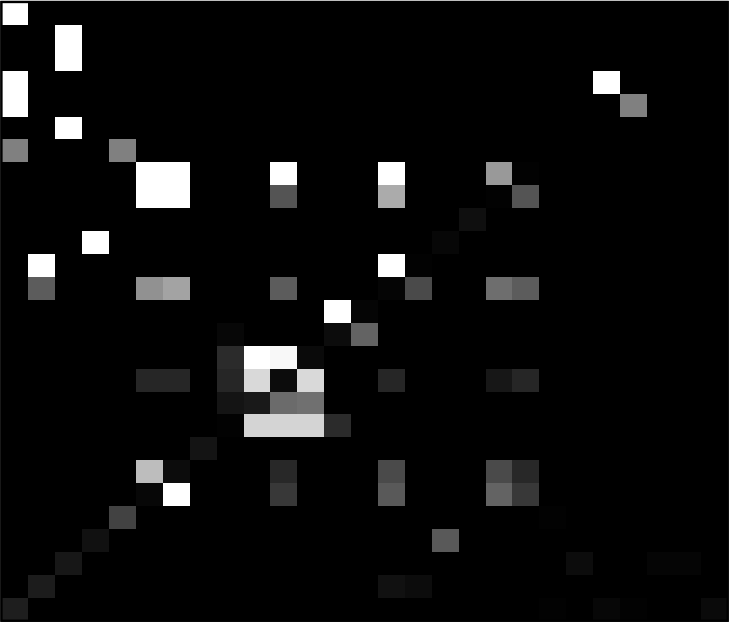
\includegraphics[width=\linewidth]{./images/genbaseHeatMap.png}
  \caption{Χάρτης Θερμότητας του συνόλου δεδομένων genbase.}
  \label{graph:genbaseHeatMap}
\endminipage\hfill
\minipage{0.47\textwidth}
  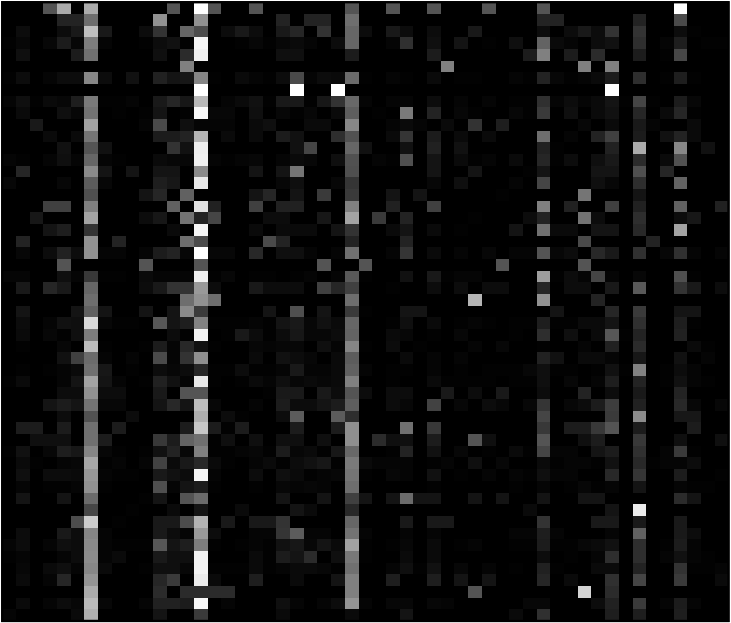
\includegraphics[width=\linewidth]{./images/enronHeatMap.png}
  \caption{Χάρτης Θερμότητας του συνόλου δεδομένων enron.}
  \label{graph:enronHeatMap}
\endminipage\hfill
\end{figure}

\item \textbf{Γράφοι Συσχετίσεων}

Αναπαριστούν δυαδικές συσχετίσεις μεταξύ των ετικετών. Κάθε ετικέτα αναπαρίσταται ως ένας κόμβος και το πάχος της ακμής που ενώνει δύο ετικέτες είναι ανάλογο της πιθανότητας $P(y_i \cap y_j)$. 

Ο γράφος συσχετίσεων των ετικετών των δειγμάτων του συνόλου scene παρουσιάζεται στο Σχήμα \ref{graph:sceneGraph}.


\begin{figure}[!htb]
 \begin{center}
    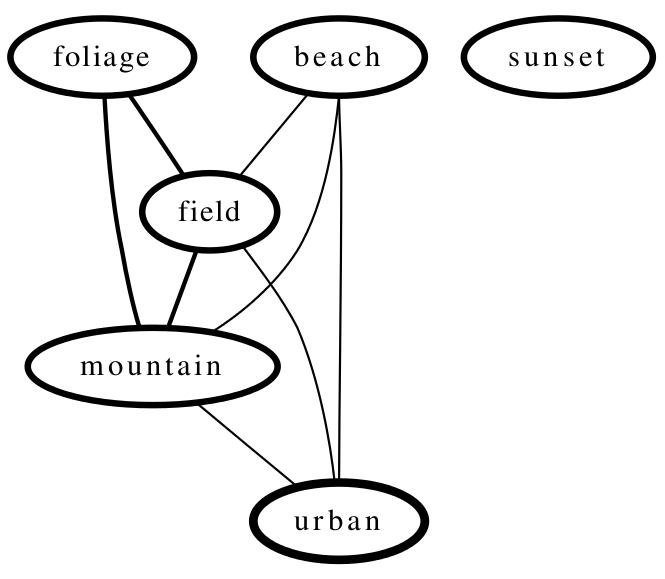
\includegraphics[scale=.3]{./images/sceneGraph.png}
  \caption{Γράφος Συσχέτισης του συνόλου δεδομένων scene.}
  \label{graph:sceneGraph}
 \end{center}
\end{figure}

\end{description}



\subsection{Ιδιότητες Πολυκατηγορικών Συνόλων Δεδομένων}
\label{subsec:mlDatasetsProperties}
Η νέα διάσταση του χώρου των ετικετών καθιστά τα διάφορα πολυκατηγορικά σύνολα δεδομένων διαφορετικά ως προς τα εσωτερικά τους χαρακτηριστικά. Δεδομένου ότι μερικά από αυτά τα χαρακτηριστικά είναι μετρήσιμα, αναφέρουμε στη συνέχεια κάποιες σχετικές, βασικές μετρικές. Στους παρακάτω ορισμούς θεωρούμε ως $D$ το σύνολο δεδομένων, $L$ το σύνολο ετικετών, $Y$ το σύνολο ετικετών με το οποίο συνδέεται ένα τυχαίο δείγμα $s \in D$ και $X$ το σύνολο των γνωρισμάτων του $D$.

\begin{description}
\item \textbf{Κατηγορική Πληθικότητα (Label Cardinality - LC)}

Η \emph{Κατηγορική Πληθικότητα} ενός συνόλου δεδομένων είναι ο μέσος όρος των ετικετών ανά δείγμα.
\begin{equation} 
LC(D)=\frac{1}{|D|} \sum_{i=1}^{|D|} |Y_i| 
\end{equation} 

\item \textbf{Κατηγορική Πυκνότητα (Label Density - LD)}

Η \emph{Κατηγορική Πυκνότητα} είναι το μέσο ποσοστό ετικετών σε ένα σύνολο δεδομένων, σε σχέση με το πλήθος των ετικετών.
\begin{equation} 
LD(D)= \frac{LC(D)}{|L|} =\frac{1}{|D|} \sum_{i=1}^{|D|} \frac{|Y_i|}{|L|} 
\end{equation} 

\item \textbf{Ποσοστό Διακριτών Συνδυασμών Ετικετών}

Είναι το ποσοστό των μοναδικών συνδυασμών ετικετών που υπάρχουν στο σύνολο των δειγμάτων: 
\begin{equation}
P_{\textsc{Dist}}(D)=\frac{\left|S|\exists(x,S) \in D \right|}{|D|} 
\end{equation}  

\item \textbf{Ποσοστό Εμφάνισης Συχνότερου Συνδυασμού Ετικετών}

Είναι ο λόγος του αριθμού των εμφανίσεων του συχνότερου συνδυασμού ετικετών προς το συνολικό αριθμό των δειγμάτων.
\begin{equation}
P_{\textsc{max}}(D)= \max_{Y|(x,Y) \in D} \frac{count(Y,D)}{|D|} 
\end{equation}
\\
Υψηλή τιμή του $P_{\textsc{max}}$ σε συνδυασμό με υψηλή τιμή του $P_{\textsc{Dist}}$ είναι ενδεικτικές ασυμμετρίας στην κατανομή των ετικετών του $D$, αντίστοιχα προς το πρόβλημα ασυμμετρίας κατανομής κλάσεων στα προβλήματα απλής κατηγοριοποίησης.

\item \textbf{Πολυπλοκότητα Συνόλου Δεδομένων (Dataset Complexity)}

ορίζεται ως το γινόμενο του αριθμού των δειγμάτων του $D$, επί το σύνολο του αριθμού των ετικετών $\abs{L}$, επί τον αριθμό των γνωρισμάτων $\abs{X}$:
\begin{equation}
\textsc{Complexity} = \abs{D} \times \abs{L} \times \abs{X}
\end{equation}
\end{description}

\subsection{Αξιολόγηση Πολυκατηγορικών Ταξινομητών}
Σε αντιδιαστολή με την απλή ταξινόμηση, η ύπαρξη της επιπλέον διάστασης των πολλαπλών ετικετών σημαίνει ότι η προσέγγιση σωστής/λανθασμένης κατηγοριοποίησης δεν είναι δυνατόν να αναπαραστήσει πλήρως την ποιότητα των ταξινομητών. Ένα δείγμα μπορεί να ταξινομείται ορθά σε μία κατηγορία, αλλά λανθασμένα σε κάποια άλλη. Υπάρχουν δύο δρόμοι που μπορούμε να ακολουθήσουμε: η \emph{αξιολόγηση βάσει ετικετών} και η \emph{αξιολόγηση βάσει συνόλου ετικετών}. 

\begin{enumerate}
\item \textbf{Αξιολόγηση βάσει ετικετών (label-based)}

Εξετάζει την κάθε ετικέτα ξεχωριστά, κάνοντας χρήση στην ουσία των αξιολογήσεων απλής ταξινόμησης. Αποτυγχάνει, όπως είναι κατανοητό, να λάβει υπόψη τις συσχετίσεις ανάμεσα στις ετικέτες και την πολυπλοκότητα του συνόλου δεδομένων, με αποτέλεσμα να είναι αρκετά επιεικής, ιδιαίτερα σε περιπτώσεις μικρού αριθμού ενεργοποιημένων ετικετών ανά δείγμα (χαμηλό label cardinality).
\item \textbf{Αξιολόγηση βάσει συνόλου ετικετών (labelset-based)}

Σε αντίθεση με την αξιολόγηση βάσει ετικετών, εκτιμά καλύτερα την ικανότητα του ταξινομητή σε ένα πολυκατηγορικό πρόβλημα, λαμβάνοντας υπόψη τις συσχετίσεις μεταξύ των ετικετών, αλλά μπορεί να αποδειχθεί υπερβολικά αυστηρή, ειδικά σε περιπτώσεις υψηλού αριθμού ενεργοποιημένων ετικετών ανά δείγμα (υψηλό label cardinality).
\end{enumerate}

Για την αξιολόγηση των πολυκατηγορικών ταξινομητών, μπορούμε να χρησιμοποιήσουμε τις, κατάλληλα τροποποιημένες \cite{li2006empirical}, μετρικές που έχουμε ήδη αναφέρει (παρ. \ref{subsub:metrics}). Έστω $L$ το σύνολο των ετικετών του συνόλου δεδομένων $D$, με δείγματα της μορφής $(x_{i}, Y_{i})$, όπου $i = 1 \dots \abs{D}$, $Y_{i} \subseteq L$, και $\hat{Y}_{i} = H(x_{i})$ η συνάρτηση πρόβλεψης του ταξινομητή. Τότε, ορίζουμε τις εξής μετρικές:

\begin{description}
\item \textbf{Ακριβής Ορθότητα (Exact Match)}

Είναι η απλούστερη και αυστηρότερη μετρική. Υπολογίζεται ως το ποσοστό των δειγμάτων που ταξινομήθηκαν ορθά για όλες τους τις κατηγορίες προς όλες τις ταξινομήσεις που έγιναν:
\begin{equation} 
\textsc{ExactMatch}=\frac{|C|}{|D|} 
\end{equation}  
όπου $C$ το σύνολο των δειγμάτων που ταξινομήθηκαν απολύτως ορθά, σε πλήρη αντιστοιχία με τις πραγματικές τους ετικέτες, δηλαδή $Y_{i} \equiv \hat{Y}_{i}$

\item \textbf{Ακρίβεια (Accuracy)}

Είναι ο μέσος όρος, υπολογισμένος με βάση όλα τα δείγματα, των λόγων του μεγέθους του συνόλου τομής προς αυτό της ένωσης των προβλεπόμενων και πραγματικών ετικετών:

\begin{equation} 
\textsc{Accuracy}(H,D)=\frac{1}{|D|} \sum_{i=1}^{|D|} \frac{\abs{Y_{i} \bigcap \hat{Y}_{i}}}{\abs{Y_i \bigcup \hat{Y}_{i}}} 
\end{equation}

\item \textbf{Πιστότητα (Precision)}

Είναι ο μέσος όρος, υπολογισμένος με βάση όλα τα δείγματα, των λόγων του μεγέθους του συνόλου τομής των προβλεπόμενων και πραγματικών ετικετών προς αυτό των προβλεπόμενων ετικετών:

\begin{equation} 
\textsc{AveragePrecision}(H,D)=\frac{1}{|D|} \sum_{i=1}^{|D|} \frac{\abs{Y_i \bigcap \hat{Y}_{i}}}{\abs{\hat{Y}_{i}}} 
\end{equation} 

\item \textbf{Ανάκληση (Recall)}

Είναι ο μέσος όρος, υπολογισμένος με βάση όλα τα δείγματα, των λόγων του μεγέθους του συνόλου τομής των προβλεπόμενων και πραγματικών ετικετών προς αυτό των πραγματικών ετικετών:

\begin{equation} 
\textsc{AverageRecall}(H,D)=\frac{1}{|D|} \sum_{i=1}^{|D|} \frac{\abs{Y_i \bigcap \hat{Y}_{i}}}{\abs{{Y}_{i}}} 
\end{equation} 

\item \textbf{Απώλεια Hamming (Hamming Loss)}
Λαμβάνει υπόψη τις εσφαλμένα θετικές (FP) και αρνητικές (FN) προβλέψεις ετικετών του ταξινομητή:

%``ξεχνά'' (FN):

\begin{equation} 
\textsc{HammingLoss}(H,D)=\frac{1}{|D|} \sum_{i=1}^{|D|} \frac{\abs{Y_{i} \varDelta \hat{Y}_{i}}}{\abs{L}} 
\end{equation}  
\\
όπου $\varDelta$ ο τελεστής της συμμετρικής διαφοράς (XOR-symmetric difference) δύο συνόλων.

\end{description}

Από τις παραπάνω μετρικές, η Ακριβής Ορθότητα, η Ακρίβεια, η Πιστότητα και η Ανάκληση είναι βασισμένες σε σύνολα ετικετών (labelset-based), ενώ η Απώλεια Hamming είναι βασισμένη σε ετικέτες (label-based).

 
\subsection{Στρατηγικές Συμπερασμού Πολυκατηγορικών Ταξινομητών}
\label{subsec:multiLabelInference}
Ονομάζουμε \textit{στρατηγική συμπερασμού} τη μέθοδο ταξινόμησης νέων, αγνώστων, δειγμάτων, δεδομένου ενός μοντέλου ταξινόμησης. Στη συνέχεια, χωρίς βλάβη της γενικότητας, υποθέτουμε ότι το χρησιμοποιούμενο μοντέλο ταξινόμησης βασίζεται σε κανόνες. 

Στα πλαίσια της μονοκατηγορικής ταξινόμησης, η διαδικασία επιλογής κλάσης είναι αρκετά απλή και άμεση. Μπορεί να περιλαμβάνει είτε επιλογή της απόφασης του βέλτιστου (ως προς κάποια μετρική αξιολόγησης) κανόνα που καλύπτει το δεδομένο δείγμα, ή ψηφοφορία μεταξύ όλων των κανόνων που το καλύπτουν. Στα πλαίσια, όμως, της πολυκατηγορικής ταξινόμησης, όπου οι ετικέτες δεν είναι αμοιβαίως αποκλειόμενες και ο αριθμός των ενεργοποιημένων ετικετών δεν είναι εκ των προτέρων γνωστός, η στρατηγική συμπερασμού καθίσταται πολυπλοκότερη, ενώ υπάρχουν εναλλακτικές στρατηγικές που μπορούν να ακολουθηθούν. Στη συνέχεια εξετάζουμε από πιο κοντά τις δύο στρατηγικές που χρησιμοποιούνται σε αυτή την εργασία.

\begin{enumerate}
\item \textbf{Επιλογή βέλτιστου κανόνα}. Με την είσοδο ενός μη επισημασμένου δείγματος, συγκεντρώνονται οι κανόνες που το καλύπτουν. Κάθε κανόνας χαρακτηρίζεται από την καταλληλότητά του (την τιμή μίας συγκεκριμένης μετρικής ή κάποιας συνάρτησης ενός ή περισσοτέρων μετρικών), πάνω στην οποία βασίζεται αυτή η μέθοδος. Απόφαση για την κάθε ετικέτα του δείγματος λαμβάνει ο πλέον κατάλληλος κανόνας από το σύνολο των κανόνων που το καλύπτουν. Στην περίπτωση που ο εν λόγω κανόνας αδιαφορεί για κάποια ετικέτα, δηλαδή δεν είναι σε θέση να παρέχει κάποια συγκεκριμένη απόφαση για αυτή, η απόφαση λαμβάνεται από τον κανόνα με την αμέσως μικρότερη καταλληλότητα κ.ο.κ.
\item \textbf{Ψηφοφορία Μέσου όρου}. Μετά τη συγκέντρωση των κανόνων που καλύπτουν το μη επισημασμένο δείγμα, ο καθένας ψηφίζει θετικά ή αρνητικά, σταθμισμένα ανάλογα με την καταλληλότητά του, για την κάθε ετικέτα, (απέχοντας από την ψηφοφορία στην περίπτωση που αδιαφορεί), αναλόγως με το τί προβλέπεται στο τμήμα της απόφασής του. Η τελική απόφαση λαμβάνεται με βάση το μέσο όρο των ψήφων για την κάθε ετικέτα. Επιπλέον, μπορεί να χρησιμοποιείται μία συνάρτηση κατωφλίου για το διαχωρισμό των ετικετών σε αυτές που είναι σχετικές και άσχετες με το δείγμα, όπως π.χ. στον αλγόριθμο RA$k$EL \cite{tsoumakas2007random}.
\end{enumerate}

Όπως έχει ήδη αναφερθεί, η επιλογή του κατωφλίου είναι σε κάποιες περιπτώσεις πολύ σημαντική, καθώς επηρεάζει άμεσα την ικανότητα κατηγοριοποίησης του ταξινομητή. Μία συνάρτηση κατωφλίου έχει τη δομή 

\begin{equation}
\hat{y_i}= f_{L,t}(w) = \left\{ \begin{matrix}1 & w_i \geq t_i \\ 0 & w_i < t_i \end{matrix}\right.                                                                                                                                        
\end{equation}  
\\
όπου $\hat{y_i}$ η πρόβλεψη του ταξινομητή για την ύπαρξη της ετικέτας $i$ και $t_i$ το κατώφλι για αυτή την ετικέτα. Για τη διευκόλυνση επιλογής μία συγκεκριμένης τιμής κατωφλίου, το διάνυσμα βεβαιοτήτων $w$ κανονικοποιείται με αποτέλεσμα τον περιορισμό των τιμών του στο διάστημα $[0, 0.5]$. Τέλος, οι περισσότερες προσεγγίσεις περιλαμβάνουν μία διαδικασία ρύθμισης του κατωφλίου, είτε εσωτερικά είτε εξωτερικά. 

Η \emph{Επιλογή με Εσωτερική Αξιολόγηση (Internal Validation - IVAL)} προσπαθεί να ορίσει μία τιμή κατωφλίου τέτοια ώστε να μεγιστοποιεί μία συγκεκριμένη μετρική, με διαδοχικούς εσωτερικούς ελέγχους ως προς τη μετρική αυτή. Η διαδικασία αυτή είναι χρονικά απαιτητική λόγω των επαναλαμβανόμενων αξιολογήσεων, ωστόσο μπορεί να βελτιωθεί από άποψη υπολογιστικής πολυπλοκότητας αξιοποιώντας το γεγονός ότι οι περισσότερες συναρτήσεις μετρικών με μεταβλητή το ίδιο το κατώφλι είναι κυρτές. Αυτό συμβαίνει αφού για μηδενικό κατώφλι, επιλέγονται πολλές ετικέτες, ενώ, καθώς αυτό αυξάνεται, αυξάνει και η ειδικότητα, αφού επιλέγονται λιγότερες ετικέτες. Προφανώς, οι μετρικές της Ακρίβειας και της Ακριβούς Ορθότητας, αρχικά αυξάνονται και στη συνέχεια μειώνονται ως κυρτές συναρτήσεις. 

Η \emph{Επιλογή με Ποσοστιαία Αποκοπή (Proportional Cut - PCUT)} ρυθμίζει εξωτερικά το κατώφλι, και προσεγγίζει την τιμή του επαναληπτικά, στοχεύοντας στην ελαχιστοποίηση της διαφοράς της πολυκατηγορικής πληθικότητας $LC$ σε ένα σύνολο δεδομένων. Λεπτομέρειες για τη μέθοδο με την οποία γίνεται η ψηφοφορία και για τις μεθόδους ρύθμισης του κατωφλίου αναφέρουμε στην Παρ. \ref{sec:multiLabelInference}.
 


